\documentclass[allowbf, simple name, palatino, a4paper]{einfart}

\nolinenumbers % Enable line numbers

%%================================
%% Import toolkit
%%================================
\usepackage{ProjLib}
\usepackage{longtable}  % breakable tables
\usepackage{hologo}     % more TeX logo

\usepackage{relsize}
\usepackage{booktabs}
\usepackage{blindtext}
\usepackage{physics}
\UseLanguage{Chinese}

%%================================
%% For typesetting code
%%================================
\usepackage{listings}
\definecolor{maintheme}{RGB}{70,130,180}
\definecolor{forestgreen}{RGB}{21,122,81}
\definecolor{lightergray}{gray}{0.99}
\lstset{language=[LaTeX]TeX,
    keywordstyle=\color{maintheme},
    basicstyle=\ttfamily,
    commentstyle=\color{forestgreen}\ttfamily,
    stringstyle=\rmfamily,
    showstringspaces=false,
    breaklines=true,
    frame=lines,
    backgroundcolor=\color{lightergray},
    flexiblecolumns=true,
    escapeinside={(*}{*)},
    % numbers=left,
    numberstyle=\scriptsize, stepnumber=1, numbersep=5pt,
    % firstnumber=last,
}
\providecommand{\meta}[1]{$\langle${\normalfont\itshape#1}$\rangle$}
\lstset{moretexcs=%
    {linenumbers,nolinenumbers,part,parttext,chapter,section,subsection,subsubsection,frontmatter,mainmatter,backmatter,tableofcontents,href,
    color,NameTheorem,CreateTheorem,cref,DNF,UseLanguage,UseOtherLanguage,AddLanguageSetting,maketitle,address,curraddr,email,keywords,subjclass,thanks,dedicatory,TheDate,ProjLib,qedhere
    }
}
\lstnewenvironment{code}%
{\setstretch{1.07}\LocallyStopLineNumbers%
\setkeys{lst}{columns=fullflexible,keepspaces=true}%
}
{\ResumeLineNumbers}
\lstnewenvironment{code*}%
{\setstretch{1.07}\LocallyStopLineNumbers%
\setkeys{lst}{numbers=left,columns=fullflexible,keepspaces=true}%
}
{\ResumeLineNumbers}

%%================================
%% tip
%%================================
\usepackage[many]{tcolorbox}
\newenvironment{tip}[1][提示]{%
    \LocallyStopLineNumbers%
    \begin{tcolorbox}[breakable,
        enhanced,
        width = \textwidth,
        colback = paper, colbacktitle = paper,
        colframe = gray!50, boxrule=0.2mm,
        coltitle = black,
        fonttitle = \sffamily,
        attach boxed title to top left = {yshift=-\tcboxedtitleheight/2, xshift=.5cm},
        boxed title style = {boxrule=0pt, colframe=paper},
        before skip = 0.3cm,
        after skip = 0.3cm,
        top = 3mm,
        bottom = 3mm,
        title={\scshape\sffamily #1}]%
}{\end{tcolorbox}\ResumeLineNumbers}

%%================================
%% Names
%%================================
\providecommand{\minimalist}{\textsf{minimalist}}
\providecommand{\minimart}{\textsf{minimart}}
\providecommand{\minimbook}{\textsf{minimbook}}
\providecommand{\einfart}{\textsf{einfart}}
\providecommand{\simplivre}{\textsf{simplivre}}

%%================================
%% Titles
%%================================
\let\LevelOneTitle\section
\let\LevelTwoTitle\subsection
\let\LevelThreeTitle\subsubsection
\numberwithin{equation}{section}
\makeatletter
\renewcommand\normalsize{%
	\@setfontsize\normalsize\@xpt\@xiipt
	\abovedisplayskip 5\p@ \@plus2\p@ \@minus5\p@
	\abovedisplayshortskip \z@ \@plus3\p@
	\belowdisplayshortskip 6\p@ \@plus3\p@ \@minus3\p@
	\belowdisplayskip \abovedisplayskip
	\let\@listi\@listI}
\makeatother
%%================================
%% Main text
%%================================
\begin{document}

\def\PackageVersion{2022/06/16}

\title{流体力学·复习要点}
\author{核工A002班 \quad 张恺}
\date{\TheDate{\PackageVersion}[only-year-month],彭康学导团}

\maketitle

\begin{abstract}
    流体力学是一门又难又简单的课,说它难是因为课本讲得难、上课学得难,说它简单是因为考试简单。有一份流传已久的复习提纲,涵盖了几乎所有的考试重点,但只有问题没有解答,在复习备考时,我根据这份提纲和课程组的PPT,整理了一份复习要点笔记,最终取得了比较好的成绩。我使用\LaTeX 重新排版了这份笔记,作了一些修订和删减,完成后由能动A001班~孙溢和王林业审核增删。为保证复习到所有考点,这份笔记比较详细,正文中不必须掌握的用“*”标出。这份笔记只能作为复习时的资料,非常不建议作为初次学习时的笔记使用。个人水平有限,欢迎批评指正。
\end{abstract}

\setcounter{tocdepth}{1}
{\setstretch{1.07}\tableofcontents}

\medskip

\LevelOneTitle{流体及其主要的物理性质}

\LevelTwoTitle{流体与连续介质模型}

\LevelThreeTitle{什么是流体}

\begin{definition}[流体]
	任意微小剪切力持续作用下发生连续变形的物质。
\end{definition}

\begin{tip}
	流体的这条定义明确地指出了其与固体的区别,简单地说,流体不能受剪。
\end{tip}

\LevelThreeTitle{流体质点}

\begin{definition}
	微小特征体,包含大量分子,具有确定的宏观统计特征。
\end{definition}

\begin{tip}
	教材上关于流体质点的描述:包含有足够多的分子因此具有确定的宏观统计特性,同时与流场的特征长度相比线性尺寸又充分小,可以看作一个几何点的流体团。
\end{tip}

\LevelThreeTitle{连续介质模型}

\begin{definition}[连续介质模型]
	流体由无限多流体质点连绵不断组成,质点之间无间隙。
\end{definition}

\LevelThreeTitle{连续介质模型的适用条件}

分子平均自由程$\ll$流动问题特征尺寸。所以对于稀薄气体,或者是激波层内,连续介质模型不再适用。

\LevelTwoTitle{流体的可压缩性}

\LevelThreeTitle{体积弹性模量}

\begin{equation}
	E_v = \rho \qty(\pdv{p}{\rho})_T = -V \qty(\pdv{p}{V})_T
\end{equation}

这是用来衡量流体可压缩性的一个物理量,流体的体积弹性模量越大,表示流体的体积越难被改变(可以理解为越硬,或者越接近于固体的性质),即流体可压缩性越小。

同样的外界条件下,液体的$E_v$比气体的$E_v$大得多,这表明气体比液体更好压缩。

特别地,如果我们认为气体是理想气体,那么根据理想气体状态方程和过程方程,就可以得到如下结论:

\begin{enumerate}
	\item 等温过程中,气体体积弹性模量$E_v = p$;
	\item 等熵过程中,气体体积弹性模量$E_v = \gamma p$,其中$\gamma = c_p / c_v$. 
\end{enumerate}

\LevelThreeTitle{不可压缩流体}

\begin{definition}[不可压缩流体]
	当流体的体积弹性模量$E_v \to \infty$,我们就称该流体不可压缩。这是一种假想的模型,实际流体都具有压缩性。
\end{definition}

一般地,液体可视作不可压缩,但水击、水下爆炸等现象中应当视作可压缩;气体可视作可压缩,但低速且温差小的气体应当视作不可压缩。

特别地,均质不可压缩流体的数学表达为$\rho = \text{const}$. 

\begin{tip}
	此处注意,流体不可压和均质并不是等价的,具体的解释需要用到物质导数相关的知识,你可以点击\ref{3.3.3}来查看。
\end{tip}

\LevelTwoTitle{流体的粘性}

\LevelThreeTitle{什么是流体的粘性}

\begin{definition}[粘性]
	流体抵抗剪切变形(相对运动)的一种固有的属性。
\end{definition}

\begin{tip}
	此处应当注意“固有属性”的涵义,当流体层间无相对运动时,流体对外不表现粘性,但不能认为此时流体失去了粘性。
\end{tip}

\LevelThreeTitle{流体粘性产生的机理及温度对粘性的影响(2021·简答)}

\begin{enumerate}
	\item 对于液体来讲,其粘性源于分子间内聚力,流体团的剪切变形改变了分子间距离,微观上,分子间引力阻止分子间距离改变,宏观上表现为内摩擦抵抗流体变形。当温度升高时,分子间内聚力变弱,于是粘性减小。
	\item 对于气体来讲,其粘性源于分子热运动,流体层间相对运动时,分子热运动导致层间发生动量交换,宏观上依然表现为内摩擦抵抗流体变形。当温度升高时,分子热运动变得更剧烈,于是粘性增大。
\end{enumerate}

\LevelThreeTitle{牛顿内摩擦定律}

\begin{definition}
	粘性切应力(单位:N/m$^2$)与层间速度梯度(角变形率)成正比,而与速度(角变形量)无关,即
	\begin{equation}
		\tau = \mu \dv{u}{y} = \mu \dv{\gamma}{t}
	\end{equation}
\end{definition}

\LevelThreeTitle{动力粘度和运动粘度}

动力粘度用$\mu$表示,单位是Pa$\cdot$s,可以反映流体真实的粘性大小,动力粘度越大,说明流体粘性越大,数学表达为

\begin{equation}
	\mu = \dfrac{\tau}{\dd{u}/\dd{y}}
\end{equation}

运动粘度用$\nu$表示,单位是m$^2$/s,不能反映流体真实的粘性大小,数学表达为

\begin{equation}
	\nu = \dfrac{\mu}{\rho}
\end{equation}

\LevelThreeTitle{牛顿流体和非牛顿流体(2021·选择)}

\begin{definition}[牛顿流体和非牛顿流体]
	符合牛顿内摩擦定律的流体就是牛顿流体,例如水,酒精等大多数纯液体和低速流动的气体;不符合牛顿内摩擦定律的流体就是非牛顿流体,例如纸浆、面糊和泥石流等。
\end{definition}

\LevelThreeTitle{理想流体}

\begin{definition}[理想流体]
	粘度为零的流体就是理想流体,即$\mu = 0$。
\end{definition}

实际流体都具有粘性。

\LevelTwoTitle{*作用在流体上的两种力}

\begin{enumerate}
	\item 质量力,作用于流体的每个质点上,大小与流体质量成正比,例如重力、惯性力。
	\item 表面力,作用于流体封闭界面上,大小与流体表面积成正比,例如压力、摩擦力。
\end{enumerate}

\LevelOneTitle{流体静力学}

\LevelTwoTitle{流体静压强}

\LevelThreeTitle{流体静压强的特点}

\begin{enumerate}
	\item 方向垂直于作用面,并指向流体内部;
	\item    静止流体任意点处静压强大小与其作用面方位无关,只是作用点位置的函数,即$p = f(x, y, z)$
\end{enumerate}

\LevelThreeTitle{理想流体压强的特点}

无论运动与否,理想流体压强都只是作用点位置的函数,$p = f(x, y, z)$。

\LevelTwoTitle{静止流体平衡微分方程}

\begin{equation}
	\vec{f} - \dfrac{1}{\rho} \nabla p = 0 \label{eq2.1}
\end{equation}

物理意义:单位质量静止流体中压力与质量力平衡。由该方程也可以推知:等压面与质量力处处垂直。

考虑在重力场中,质量力只有$-\va*{z}$方向的重力,于是有

\begin{equation}
	\dv{p}{z} = -\rho g
\end{equation}

若是均质不可压缩流体,则有

\begin{equation}
	p_1 = p_2 + \rho g h
\end{equation}

这个式子表明:

\begin{enumerate}
	\item 铅垂方向上,压强与淹深呈线性关系;
	\item 等压面为水平面。
\end{enumerate}

\LevelTwoTitle{*帕斯卡原理}

\begin{theorem}[帕斯卡原理]
	充满液体的连通器内,一点的压强变化可瞬时传递到整个连通器内。
\end{theorem}

\begin{tip}
	注意此处可以与第11章的微弱扰动波联系起来。实际上压强变化属于微弱扰动,在流体中以音速传播,若认为液体不可压缩,即$E_v \to \infty$,根据$a = \sqrt{E_v/\rho}$可得其传播速度为无穷大。这就是帕斯卡原理只适用于\textbf{充满液体}的连通器内的原因。
\end{tip}

\LevelTwoTitle{三种压强}

\begin{enumerate}
	\item 绝对压强$p$,以完全真空状态为零压强计量的压强;
	\item 计示压强$p_m$,以当地大气压强为基准计量的压强,$p_m = p - p_a$;
	\item 真空压强$p_v$,绝对压强低于当地大气压强时的计示压强的绝对值,$p_v = p_a - p$。
\end{enumerate}

\LevelTwoTitle{*三种测压计的特点}

\begin{enumerate}
	\item 单管测压计
	\begin{enumerate}
		\item 被测压强不能太大;
		\item 只能测量液体压强;
		\item 被测压强必须高于当地大气压强,即无法测得真空压强。
	\end{enumerate}
    \item U型管测压计
    \begin{enumerate}
    	\item 测量范围比较大;
    	\item 可以测液体、气体压强;
    	\item 可以测真空压强;
    	\item 指示液不能与被测液掺混。
    \end{enumerate}
    \item 倾斜式微压计
    放大了测量距离,提高了测量精度,应注意计算方法。
\end{enumerate}

\begin{tip}
	对于本章,必须要掌握的计算题就是较复杂的组合管测压计的计算,可以参考课后题练习。
\end{tip}

\LevelOneTitle{流体运动学基础}

\LevelTwoTitle{描述流体运动的两种方法}

\LevelThreeTitle{拉格朗日方法}

着眼于流体质点,描述每个质点自始至终的运动规律,此方法下对于任一物理量$\eta$的数学表达可以写作

\begin{equation}
	\eta = \eta(a, b, c, t)
\end{equation}

其中$(a, b, c)$是流体质点初始时刻位置坐标,$t$是时刻,它们统称为拉格朗日变数。

\LevelThreeTitle{欧拉方法(使用更广泛)}

着眼于空间点,描述空间某点流体物理量随时间的变化规律及由一点转向另一点时该量的变化,此方法下对于任一物理量$\eta$的数学表达可以写作

\begin{equation}
	\eta = \eta(x, y, z, t)
\end{equation}

其中$(x, y, z)$是空间点的位置坐标,$t$是时刻,它们统称为欧拉变数。

\begin{tip}
	可以这样理解,想象一个任意小的监测器,对于两种研究方法:
	\begin{itemize}
		\item 拉格朗日方法是把监测器放置在流体质点上,在流动过程中监测器始终跟着流体质点运动,能反映这个流体质点从头到尾的物理量变化;
		\item 欧拉方法是把监测器放置在一个空间点上,在流动过程中监测器不动,能反映流过这个空间点的流体质点的物理量变化。
		\item 举个简单的例子,就拿测速度来说,依据拉格朗日方法,就应该在流体质点上安置速度传感器,而依据欧拉方法,则应该在固定空间位置上安置风速仪。
	\end{itemize}
\end{tip}

\LevelTwoTitle{几个重要的概念}

\begin{enumerate}
	\item 定常
	\begin{equation}
		\pdv{\eta}{t} = 0
	\end{equation}
    \item 均匀
    \begin{equation}
    	\pdv{\eta}{x} = \pdv{\eta}{y} = \pdv{\eta}{z} = 0
    \end{equation}
    \item $n$维流动\\
    速度场为$n$个空间坐标的函数。
    \item 迹线\\
    流体质点在空间运动时描绘出的轨迹,是同一质点,不同时刻空间位置的连线,是实际存在的线,随时间增长而延长,属于拉格朗日方法下的概念,数学表达为
    \begin{equation}
    	\dfrac{\dd{x}}{u} = \dfrac{\dd{y}}{v} = \dfrac{\dd{z}}{w} = \dd{t}
    \end{equation}
    \item 流线\\
    某瞬时流场中一条假想的曲线,曲线上各点速度方向与该点处切线方向重合,是不同质点,同一时刻空间位置的连线,其走向和疏密反映了某瞬时流体速度方向和大小(流线密的地方流速大),属于欧拉方法下的概念,数学表达为
    \begin{equation}
    	\vec{V} \times \dd{\vec{l}} \text{~或~} \dfrac{\dd{x}}{u} = \dfrac{\dd{y}}{v} = \dfrac{\dd{z}}{w}
    \end{equation}
    一般情况下,流线不能相交和转折,但奇点和驻点处除外。
    \item *脉线\\
    相继通过流场同一空间点的流体质点在同一瞬时的连线,反映流场结构、流动特点,可以用染色剂通过细管掺入流体中,染色剂的轨迹就是脉线,故也可以把脉线称为染色线。
    \begin{tip}
    	定常流动时,流线形状位置不随时间改变,迹线、流线和脉线三线合一。
    \end{tip}
    \item *流管\\
    在流场中作一封闭且不自相交的曲线,在某瞬时通过该曲线上的流线构成的管状表面。显然,定常流动时,流管的形状也不改变。
    \item *过流断面\\
    与总流所有流线垂直的截面。
\end{enumerate}

\LevelTwoTitle{物质导数}

\LevelThreeTitle{物质导数的数学表达、物理意义和理解}

任意物理量$\eta$的物质导数

\begin{equation}
	\dfrac{\mathrm{D}\eta}{\mathrm{D}t} = \pdv{\eta}{t} + \vec{V} \cdot \nabla \eta 
\end{equation}

各项的物理意义如下:

\begin{enumerate}
	\item $\dfrac{\mathrm{D}\eta}{\mathrm{D}t}$表示流体质点的物理量$\eta$随时间的变化率,称为物质导数(或质点导数、随体导数);
	\vskip 0.1cm
	\item $\displaystyle \pdv{\eta}{t}$表示空间点上的物理量$\eta$随时间的变化率,反映了物理量场的非定常性,称为局部导数(或当地导数);
	\item $\vec{V} \cdot \nabla \eta$表示流体质点在非均匀的物理量场运动引起的$\eta$的变化率,称为位变导数(或对流导数)。
\end{enumerate}

\begin{tip}
	物质导数是一个非常难理解的概念,可以通过下面这个典型的例子来理解。
	\begin{enumerate}
		\item 想象这样一个情景:某人傍晚从山脚出发去爬山,当他到达山顶时已经是凌晨了,在爬山的过程中,他感到气温变低了,这是物质导数。他有这样的感觉,是两方面的因素决定的。
		\item 一方面,时间从傍晚推移到凌晨,气温会降低,这是当地气温随时间变化导致的,反映了气温的非定常性,这就是局部导数(当地导数);
		\item 另一方面,从山脚到山顶,在这个运动过程中,他所处的海拔变高,气温也是降低的,这是他在非均匀的温度分布空间上的运动导致的,这就是位变导数(对流导数);
		\item 物质导数就是综合考虑了这两方面的结果,同时把拉格朗日方法和欧拉方法联系了起来。
	\end{enumerate}
\end{tip}

\LevelThreeTitle{物质导数描述加速度}

\begin{equation}
	\vec{a} = \dfrac{\mathrm{D}\vec{V}}{\mathrm{D}t} = \pdv{\vec{V}}{t} + \vec{V} \cdot \nabla \vec{V}
\end{equation}

各项物理意义不再赘述,这时要注意两个问题。

\begin{enumerate}
	\item 速度场定常$\Leftrightarrow \displaystyle \pdv{\vec{V}}{t} = 0$;
	\vskip 0.1cm
	\item 速度场均匀$\Rightarrow \vec{V} \cdot \nabla \vec{V} = 0$,但反过来不成立。
\end{enumerate}

\LevelThreeTitle{物质导数描述不可压缩流体}\label{3.3.3}

\begin{definition}[不可压缩流体]
	运动过程中流体质点密度不变的流体叫不可压缩流体,数学表达为
	\begin{equation}
		\dfrac{\mathrm{D}\rho}{\mathrm{D}t} = 0
	\end{equation}
\end{definition}

均质流体的数学表达为$\nabla \rho = 0$,均质不可压缩流体的数学表达为$\rho = \text{const}$。

显然,$\dfrac{\mathrm{D}\rho}{\mathrm{D}t} = 0 \nLeftrightarrow \nabla \rho = 0$,即流体不可压和均质并不等价,进一步,均质不可压缩流体也不能简单地描述为不可压缩流体。

\LevelTwoTitle{流体微团的运动}

\LevelThreeTitle{分类}

流体微团的运动分为三种:平动、变形(线变形和角变形)、旋转。

\LevelThreeTitle{数学描述}

\begin{enumerate}
	\item 平动的描述上文已说明;
	\item 线变形
	\begin{enumerate}
		\item *相对伸长率
		\begin{equation*}
			\pdv{u}{x}, \pdv{v}{y}, \pdv{w}{z}
		\end{equation*}
	    \item 相对体积膨胀率
	    \begin{equation*}
	    	\dfrac{1}{\delta \tau} \cdot \dfrac{\mathrm{D}(\delta \tau)}{\mathrm{D}t} = \pdv{u}{x} + \pdv{v}{y} + \pdv{w}{z} = \nabla \cdot \vec{V} 
	    \end{equation*}
        不可压缩流体也可以表达为$\nabla \cdot \vec{V} = 0$,这是拉格朗日方法下推得的。
	\end{enumerate}
    \item *角变形率
    \begin{equation*}
    	\dfrac{\mathrm{D}\gamma_{xy}}{\mathrm{D}t} = \pdv{u}{y} + \pdv{v}{x}, \dfrac{\mathrm{D}\gamma_{yz}}{\mathrm{D}t} = \pdv{v}{z} + \pdv{w}{y}, \dfrac{\mathrm{D}\gamma_{zx}}{\mathrm{D}t} = \pdv{w}{x} + \pdv{u}{z}
    \end{equation*}
    \item 旋转角速度
    \begin{equation*}
    	\vec{\omega} = \dfrac{1}{2} \nabla \times \vec{V}
    \end{equation*}
    无旋$\Leftrightarrow \vec{\omega} = 0$
\end{enumerate}

\LevelTwoTitle{*连续性原理}\label{3.5}

对于连续性原理,有两种表述:
\begin{enumerate}
	\item 拉格朗日方法:系统包含的质量在运动过程中不变;
	\item 欧拉方法:净流出控制体的流体质量 = 控制体减少的流体质量。
\end{enumerate}

\LevelThreeTitle{连续方程}

\begin{equation}
	\pdv{\rho}{t} + \nabla \cdot (\rho \vec{V}) = 0
\end{equation}

这是在欧拉方法下推得的,是质量守恒定律的表现,是流动存在的必要条件,对理想和粘性流体均适用。

\begin{enumerate}
	\item 若是定常流动,则有$\nabla \cdot (\rho \vec{V}) = 0$,表示净流出单位控制体的质量流量为0;
	\item 若是不可压缩流动,则有$\nabla \cdot \vec{V} = 0$,表示净流出单位控制体的体积流量为0。
\end{enumerate}

\begin{tip}
	可以看到,在欧拉方法下推得的不可压缩流动表达式和拉格朗日方法下的结果一致,这说明了两种研究方法在结果上的共通性,但应注意二者的物理意义并不相同。
	
	对于同样形式的$\nabla \cdot \vec{V} = 0$,
	
	\begin{enumerate}
		\item 拉格朗日方法认为,这表示流体微团的相对体积膨胀率为0;
		\item 欧拉方法认为,这表示净流出单位控制体的体积流量为0。
	\end{enumerate}
\end{tip}

\LevelThreeTitle{一维定常流动连续方程}

一般来讲,在后续章节遇到的计算中用到的连续方程都属于此类。

\begin{enumerate}
	\item 不可压缩流体,体积流量守恒,$Q = \text{const} \Rightarrow \overline{V}_1A_1 = \overline{V}_2A_2$;
	\item 可压缩流体,质量流量守恒,$\dot{m} = \text{const} \Rightarrow \rho_1\overline{V}_1A_1 = \rho_2\overline{V}_2A_2$
\end{enumerate}

\begin{tip}
	依照课程设置,只有在第11章涉及可压缩流体,会用到质量流量守恒,其余章节全部使用体积流量守恒。
\end{tip}


\LevelOneTitle{理想流体运动基础}

\LevelTwoTitle{雷诺数$Re$}

\begin{equation*}
	Re = \dfrac{\rho V L}{\mu}
\end{equation*}

雷诺数是惯性力和粘性力之比,将流动视作无粘流动(理想流动)的必要条件是$Re \gg 1$。

\LevelTwoTitle{理想流体平衡微分方程(欧拉方程)}

\begin{equation}
	\dfrac{\mathrm{D} \vec{V}}{\mathrm{D} t} = \vec{g} - \dfrac{1}{\rho} \nabla p \label{eq4.2}
\end{equation}

本质是牛顿第二定律的应用,压力和重力的合力产生加速度。特别地,若流体加速度为0,这就是第2章中的式\ref{eq2.1},成为静止流体平衡微分方程。

\LevelTwoTitle{沿流线的伯努利方程}

\begin{equation}
	\dfrac{V^2}{2} + gz + \dfrac{p}{\rho} = \text{const}
\end{equation}

\begin{enumerate}
	\item 物理意义
	\begin{enumerate}
		\item $\dfrac{V^2}{2}$表示单位质量流体的动能;
		\vskip 0.1cm
		\item $gz$表示单位质量流体的重力势能;
		\vskip 0.1cm
		\item $\dfrac{p}{\rho}$表示单位质量流体的压力能;
		\vskip 0.1cm
		\item 整个式子表示单位质量流体的机械能沿流线守恒。
	\end{enumerate}
	\item 几何意义(2021·简答)
	\begin{equation}
		\dfrac{V^2}{2g} + z + \dfrac{p}{\rho g} = \text{const}
	\end{equation}
	\begin{enumerate}
		\item $\dfrac{V^2}{2g}$表示速度水头,是不考虑阻力时流体以速度$V$垂直上射的高度;
		\vskip 0.1cm
		\item $z$表示位置水头,是流体质点相对于基准面的位置高度;
		\vskip 0.1cm
		\item $\dfrac{p}{\rho g}$表示压强水头,是产生压强$p$所需的流体住高度。
		\vskip 0.1cm
		\item 整个式子表示理想流体沿同一条流线的总能头为常数,总能头线是水平直线。
	\end{enumerate}
    \item 适用条件(2021·简答)
    \begin{enumerate}
    	\item 理想均质不可压;
    	\item 定常;
    	\item 质量力有势且只有重力;
    	\item 沿同一条流线;
    	\item 无其他能量输入输出。
    \end{enumerate}
\end{enumerate}

\LevelTwoTitle{伯努利方程的应用}

毕托管、虹吸管、文丘里流量计。

\begin{tip}
	本章可能涉及简答题(考查流线伯努利方程的物理意义、几何意义、适用条件,这些一定要清楚)和计算题(伯努利方程的应用),出计算题的概率小一些,会做作业题即可。
\end{tip}


\LevelOneTitle{粘性流动基础}

\LevelTwoTitle{粘性流体一点应力状态}

对于理想流体,一点应力$p = p(x, y, z)$,方向垂直于作用面并指向流体内部,大小与作用面方位无关,只是作用点位置的函数。

对于粘性流体则不然,其一点应力分为法向应力$\sigma_n$和切向应力$\tau_n$,大小与作用面有关。

\LevelTwoTitle{*N-S方程}

\LevelThreeTitle{本构方程}

本构方程反映应力与变形率的关系。

\LevelThreeTitle{N-S方程}

N-S方程是牛顿第二定律应用于流体微团,物理意义是流体微团所受重力和表面力的合力等于流体微团质量乘加速度。

可以了解不可压流体的N-S方程的形式:

\begin{equation}
	\dfrac{\mathrm{D} \vec{V}}{\mathrm{D} t} = \vec{g} - \dfrac{1}{\rho} \nabla p + \nu \nabla^2 \vec{V}
\end{equation}

若是理想流体,则去掉粘性项,就成为欧拉方程(式\ref{eq4.2}),即

\begin{equation*}
	\dfrac{\mathrm{D} \vec{V}}{\mathrm{D} t} = \vec{g} - \dfrac{1}{\rho} \nabla p
\end{equation*}

若流体静止,则加速度为0,就成为静止流体平衡微分方程(式\ref{eq2.1})的形式,即

\begin{equation*}
	0 = \vec{g} - \dfrac{1}{\rho} \nabla p
\end{equation*}

\LevelTwoTitle{流动状态}

\LevelThreeTitle{不同流态的特点}

流体流态分为:层流、转捩和湍流。

\begin{enumerate}
	\item 层流,分层流动,质点轨迹光滑,流动稳定;
	\item 转捩,层与层之间开始掺混;
	\item 湍流,层与层之间剧烈掺混,质点轨迹杂乱无章,流体做复杂无规则的随机运动,属于三维非定常有旋运动。
\end{enumerate}

\LevelThreeTitle{雷诺数}

雷诺数$Re$是决定流态的判据,物理意义是惯性力和粘性力之比,数学表达式为

\begin{equation}
	Re = \dfrac{\rho V L}{\mu} = \dfrac{V L}{\nu}
\end{equation}

其中,$V$是特征速度,$L$是特征长度。

\begin{table}[H]
	\centering
	\begin{tabular}{ccc}
		\toprule[1pt]
		流动问题 & 特征速度 & 特征长度 \\
		\hline
		圆管内流 & 管内流速$V$ & 圆管内径$D$ \\
		平板边界层 & 无穷来流速度$U_{\infty}$ & 距前缘距离$x$或边界层厚度$\delta$\\
		\bottomrule[1pt]
	\end{tabular}
    \caption{不同流动问题有不同的特征物理量}
\end{table}

雷诺数$Re$判断流态的原理(容易考简答题):

\begin{enumerate}
	\item $Re$较小时,粘性力影响显著,扰动受粘性阻尼作用衰减,此时为层流;
	\item $Re$较大时,惯性力影响显著,惯性力对扰动的放大作用远超粘性阻尼作用,此时为湍流。
\end{enumerate}

\LevelTwoTitle{三种解析解}

可以不掌握具体表达式,但要知道速度和切应力分布的图形以及最大速度和平均速度的关系。

\begin{enumerate}
	\item 平面泊肃叶流动,$u_{\text{max}} = 1.5 \overline{V}$。
	\begin{figure}[H]
		\centering
		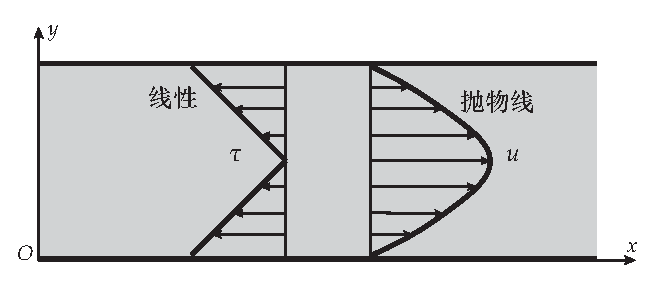
\includegraphics[scale=0.6]{figures/平面泊肃叶.eps}
		\caption{平面泊肃叶流动的速度和切应力分布}
	\end{figure}
	\item 平面库埃特-泊肃叶流动,斜直线:$\displaystyle \pdv{p}{x} = 0$;斜直线右侧(斜直线+抛物线,顺压梯度):$\displaystyle \pdv{p}{x} < 0$;斜直线左侧(斜直线$-$抛物线,逆压梯度):$\displaystyle \pdv{p}{x} > 0$。
	\begin{figure}[H]
		\centering
		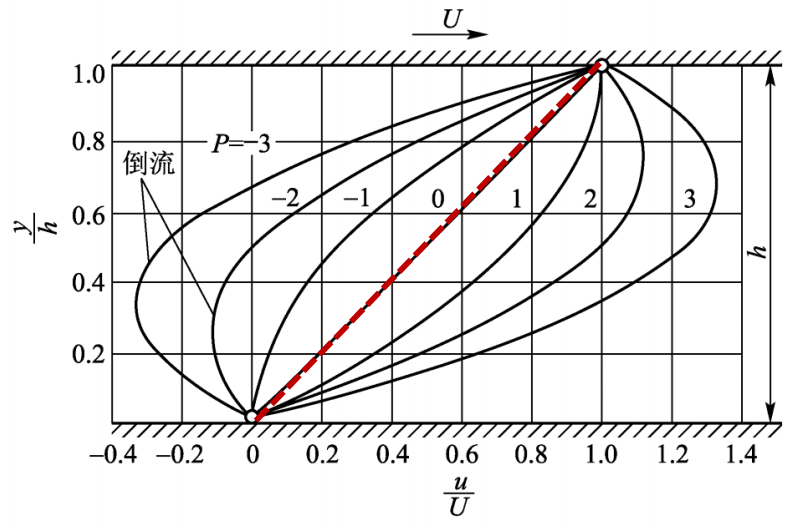
\includegraphics[scale=0.35]{figures/平面库埃特.png}
		\caption{平面库埃特-泊肃叶流动的速度分布}
	\end{figure}
	\item 圆管内泊肃叶流动,$V_{z_{\text{max}}} = 2 \overline{V}_z$。
	\begin{figure}[H]
		\centering
		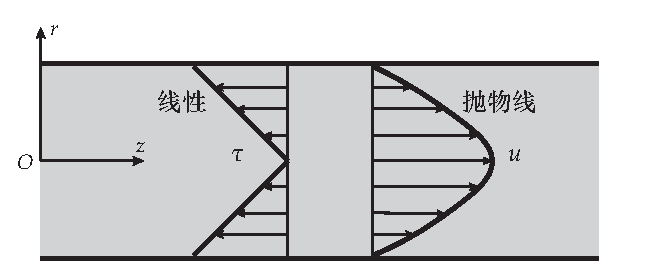
\includegraphics[scale=0.6]{figures/圆管泊肃叶.eps}
		\caption{圆管内泊肃叶流动的速度和切应力分布}
	\end{figure}
\end{enumerate}

\LevelTwoTitle{湍流物理量}

\begin{enumerate}
	\item 瞬时物理量$\eta$;
	\item 时均物理量$\displaystyle \overline{\eta} = \dfrac{1}{T} \int_{t_0}^{t_0 + T} \eta(t) \dd{t}$;
	\item 脉动物理量$\eta' = \eta - \overline{\eta}$。
\end{enumerate}

脉动物理量的时均值(2021·选择)

\begin{equation}
	\overline{\eta'} = \overline{\eta - \overline{\eta}} = \overline{\eta} - \overline{\eta} = 0
\end{equation}

\LevelTwoTitle{*雷诺应力}

\begin{enumerate}
	\item 层流切应力
	\begin{equation*}
		\tau = \mu\dv{u}{y}
	\end{equation*}
    \item 湍流切应力
    \begin{equation}
    	\tau = \mu\dv{u}{y} - \rho \overline{u' v'}
    \end{equation}
\end{enumerate}

其中,$\rho \overline{u' v'}$就是雷诺应力,由流体微团脉动导致动量横向传递引起,是流体微团在$x$方向上动量的时均值。

对于圆管湍流,在层流底层中,分子粘性应力$\displaystyle \mu \dv{u}{y}$占主导地位;在湍流核心区,雷诺应力$\rho \overline{u' v'}$占主导地位。

\LevelTwoTitle{圆管湍流}

只需要定性了解不同区域速度分布的情况,不必掌握表达式。

\begin{enumerate}
	\item 近壁区层流底层,速度为线性分布;
	\item 湍流核心区,速度为对数分布或幂律分布,随着流速的增加,幂律分布中的$n$也增大,速度分布变得均匀。
\end{enumerate}


\LevelOneTitle{流体动力学积分方程分析}

\begin{tip}
	本章中雷诺输运公式和原始形式的连续方程、能量方程和动量方程的数学表达式均不需要掌握,重点是理解物理意义和用控制体描述系统的研究思想,以及熟练掌握解题方法(只掌握做题方法当然也可以)。本章考计算题的概率非常大。
\end{tip}

\LevelTwoTitle{系统和控制体}

\begin{definition}[系统]
	某一确定流体质点集合的总体,与外界无质量交换,随流体质点运动,边界形状、包围空间大小随流体质点运动而变化。
\end{definition}

\begin{definition}[控制体]
	流场中某一确定的空间区域,与外界有质量交换,空间位置相对参照系不变,有确定的边界形状和包围空间大小。
\end{definition}

\LevelTwoTitle{*雷诺输运公式}

\begin{equation}
	\dfrac{\mathrm{D} \varPhi_{\text{sys}}}{\mathrm{D} t} = \pdv{t} \int_{\text{CV}} \phi \dd{\tau} + \int_{\text{CS}} \phi \vec{V} \cdot \vec{n} \dd{S}
\end{equation}

物理意义

\begin{enumerate}
	\item $\dfrac{\mathrm{D} \varPhi_{\text{sys}}}{\mathrm{D} t}$表示系统物理量$\varPhi_{\text{sys}}$随时间的变化率;
	\vskip 0.1cm
	\item $\displaystyle \pdv{t} \int_{\text{CV}} \phi \dd{\tau}$表示控制体物理量$\varPhi$对时间的变化率,反映流场的非定常性;
	\vskip 0.1cm
	\item $\displaystyle \int_{\text{CS}} \phi \vec{V} \cdot \vec{n} \dd{S}$表示控制体物理量$\varPhi$流出控制体的净流率,反映流场的非均匀性,体现系统位置、体积随时间改变。
	\item 整个公式是欧拉方法下采用与控制体相关的物理量描述系统的物质导数。
\end{enumerate}

\begin{tip}
	本质上,雷诺输运公式(积分形式,研究系统物理量和控制体物理量之间的关系)和物质导数公式(微分形式,研究流体质点物理量和空间点物理量之间的关系)是等价的。
\end{tip}

\LevelTwoTitle{控制方程}

\LevelThreeTitle{连续方程}

\begin{equation}
	\dfrac{\mathrm{D} m}{\mathrm{D} t} = \pdv{t} \int_{\text{CV}} \rho \dd{\tau} + \int_{\text{CS}} \rho \vec{V} \cdot \vec{n} \dd{S} 
\end{equation}

连续方程依然是质量守恒定律的应用,每一项的物理意义可以依照雷诺输运公式的解释写出,对于控制体来说,单位时间CV内流体质量增加与净流出CV的流体质量流量之和为0,可以回顾第\ref{3.5}节中的欧拉连续性原理。

\textbf{计算题中只需要掌握}在均布、定常条件下的简化形式:
\begin{equation}
	\begin{split}
		\dot{m} &= \rho V A = \text{const} \\
		Q &= V A = \text{const}
	\end{split}
\end{equation}

\LevelThreeTitle{能量方程}

\begin{equation}
	\dfrac{\mathrm{D} E}{\mathrm{D} t} = \dot{Q} + \dot{W} = \pdv{t} \int_{\text{CV}} \rho e \dd{\tau} + \int_{\text{CS}} \rho e \vec{V} \cdot \vec{n} \dd{S} 
\end{equation}

\textbf{计算题中只需要掌握}总流伯努利方程:

\begin{equation}
	z + \dfrac{p}{\rho g} + \dfrac{\alpha \overline{V}^2}{2 g} = \text{const}
\end{equation}

其中,$\alpha$为动能修正系数,反映过流断面速度分布不均匀性,在本章计算题中取1即可,实际数学表达式为
\begin{equation}
	\alpha = \dfrac{\displaystyle \int_{A} V^3 \dd{A}}{\overline{V}^3 A}
\end{equation}

总流伯努利方程的适用条件
\begin{enumerate}
	\item 理想不可压;
	\item 定常;
	\item 质量力有势且只有重力;
	\item 两过流断面必须是缓变流过流断面;
	\item 两过流断面间无能量输入输出。
\end{enumerate}

\begin{definition}[缓变流]
	流线近似于互相平行的直线的流动称为缓变流,缓变流过流断面上流体重力势能和压力能之和为常数,动压分布和静压分布相同,即
	\begin{equation}
		z + \dfrac{p}{\rho g} = \text{const}
	\end{equation}
\end{definition}

\LevelThreeTitle{动量方程}

\begin{equation}
	\sum \vec{F} = \pdv{t} \int_{\text{CV}} \rho \vec{V} \dd{\tau} + \int_{\text{CS}} \rho \vec{V} \vec{V} \cdot \vec{n} \dd{S} 
\end{equation}

\textbf{计算题中只需要掌握}

\begin{equation}
	\sum \vec{F} = \sum \qty(\dot{m}_i \vec{V}_i)_{\text{out}} - \sum \qty(\dot{m}_i \vec{V}_i)_{\text{in}}
\end{equation}

其中,$\dot{m} = \rho V A$。动量正负号规则是:与坐标方向一致为正,相反为负。

\LevelTwoTitle{例题练习}

\begin{example}
	如图,一圆盘中心有一锐边圆孔,速度为$V$的水射流撞击在圆盘中心,通过圆盘中心孔的射流速度也是$V$。试求需施加多大的力才能保持圆盘在空间位置不变。设$V = 5$ m/s,$D = 100$ mm,$d = 20$ mm。
	
	\begin{figure}[H]
		\centering
		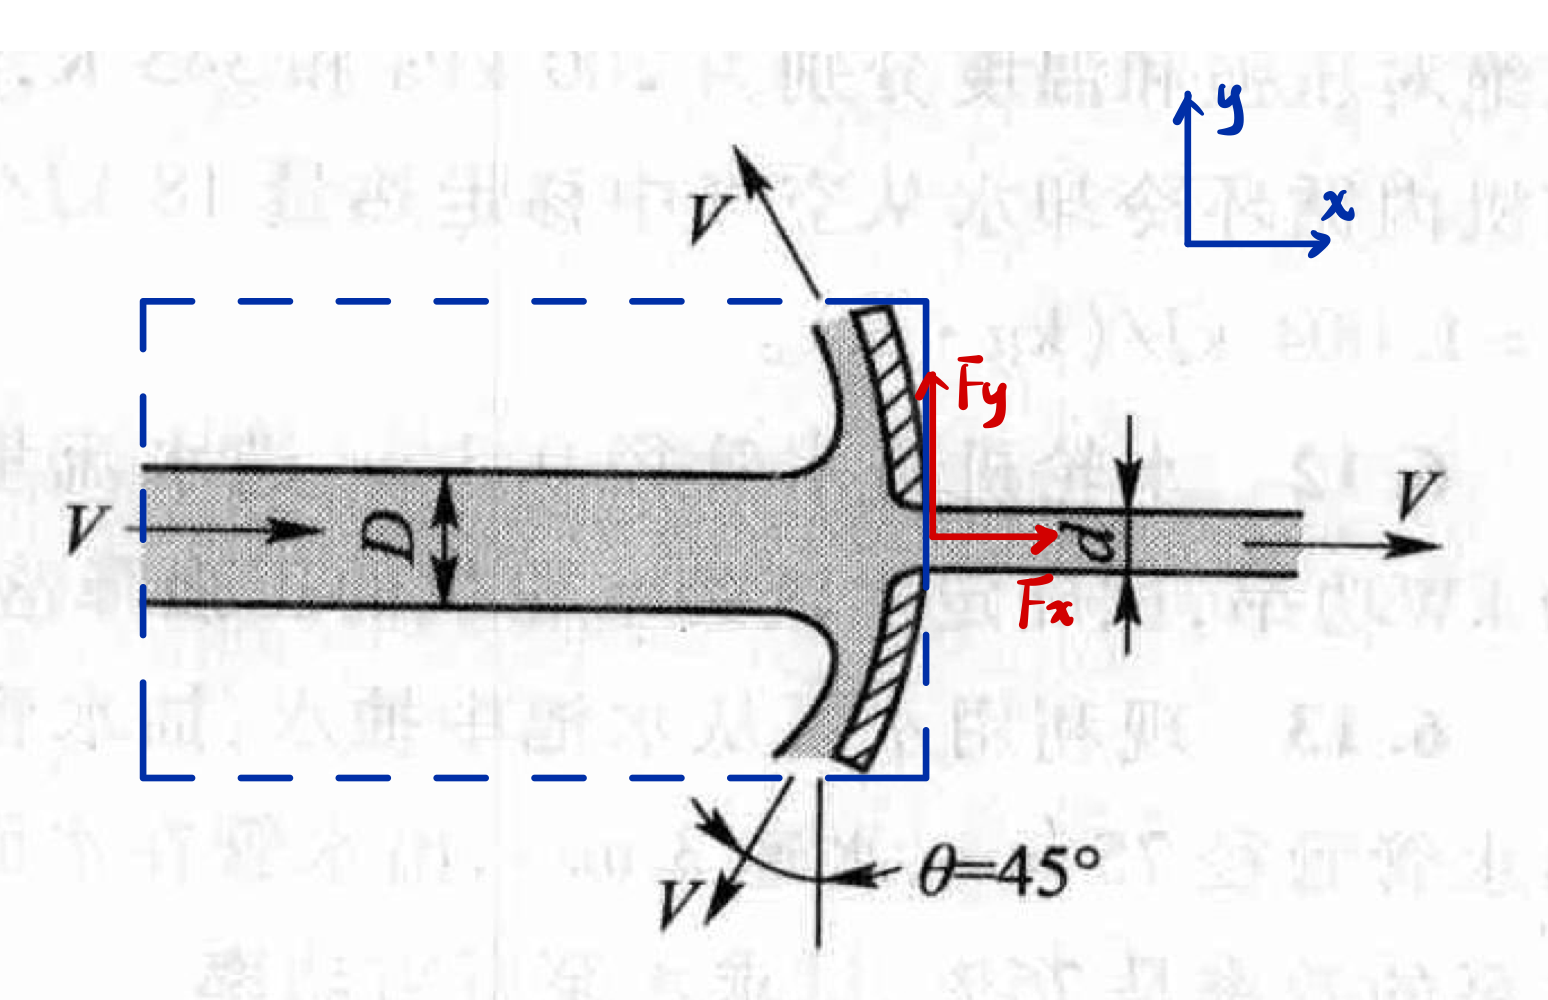
\includegraphics[scale=0.12]{figures/C6-fig3.png}
		\caption{例6.4图}
	\end{figure}
	
	设控制体上下两出口的截面积为$A_1$,根据连续方程,有
	\begin{equation*}
		V \cdot \dfrac{1}{4} \pi D^2 = 2 V \cdot A_1 + V \cdot \dfrac{1}{4} \pi d^2
	\end{equation*}
	
	解得
	\begin{equation*}
		A_1 = \dfrac{1}{8} \pi \qty(D^2 - d^2) = \dfrac{1}{8} \pi \qty(0.1^2 - 0.02^2) \mathrm{~m}^2 = 3.770 \times 10^{-3} \mathrm{~m}^2
	\end{equation*}
	
	列动量方程
	\begin{align*}
		F_x &= \sum \qty(\dot{m}_i V_{xi})_{\mathrm{out}} - \sum \qty(\dot{m}_i V_{xi})_{\mathrm{in}} \\
		&= \qty(\rho V^2 \cdot \dfrac{1}{4} \pi d^2 - 2 \rho V^2 \sin 45^{\circ} \cdot A_1) - \rho V^2 \cdot \dfrac{1}{4} \pi D^2 \\
		&= \qty(1000 \times 25 \times \dfrac{1}{4} \pi 0.02^2 - 2 \times 1000 \times \dfrac{25}{\sqrt{2}} \times 3.770 \times 10^{-3}) - 1000 \times 25 \times \dfrac{1}{4} \pi \times 0.1^2 \mathrm{~N} \\
		&= -321.8 \mathrm{~N}
	\end{align*}
	
	负号表示$F_x$方向与$x$轴正方向相反,即$F_x$的方向是水平向左。
	\begin{align*}
		F_y &= \sum \qty(\dot{m}_i V_{yi})_{\mathrm{out}} - \sum \qty(\dot{m}_i V_{yi})_{\mathrm{in}} \\
		&= \qty(\rho V^2 \cos 45^{\circ} \cdot A_1 - \rho V^2 \cos 45^{\circ} \cdot A_1) - 0 \\
		&= 0
	\end{align*}
	
	综上所述,需施加一个水平向左且大小为321.8 N的力。
\end{example}

\begin{example}
	如图,小车在射流冲击下以恒定速度$U$沿水平方向运动,固定在车上的叶片的偏转角为$\theta$。射流的绝对速度为$V$,试求叶片受到的合力及产生的功率大小,并证明$U = V/3$时该功率最大。
	
	\begin{figure}[H]
		\centering
		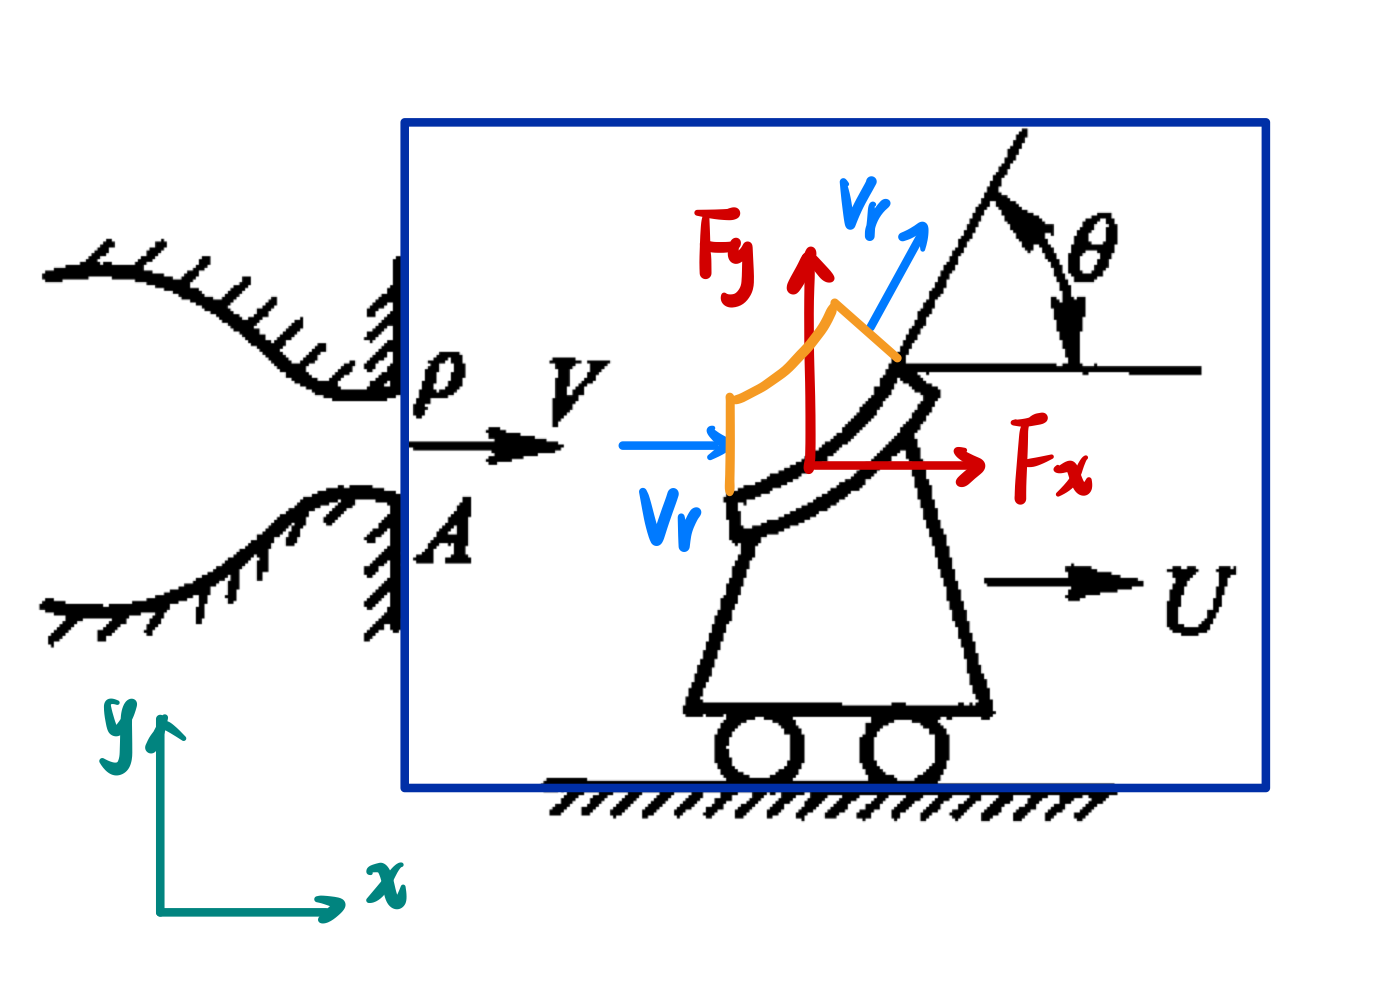
\includegraphics[scale=0.12]{figures/C6-fig2.png}
	\end{figure}

    建立如图所示的坐标系,令其相对于小车静止,则相对速度$V_r = V - U$。
    
    列动量方程
    \begin{align*}
    	&F_x = \sum \qty(\dot{m}_i V_{xi})_{\mathrm{out}} - \sum \qty(\dot{m}_i V_{xi})_{\mathrm{in}} = \rho V_r^2 \cos \theta A - \rho V_r^2 A \\
    	&F_y = \sum \qty(\dot{m}_i V_{yi})_{\mathrm{out}} - \sum \qty(\dot{m}_i V_{yi})_{\mathrm{in}} = \rho V_r^2 \sin \theta A
    \end{align*}
    
    由牛顿第三定律,得到叶片受到的力为
    \begin{align*}
    	&F_x' = \rho \qty(V-U)^2 A \qty(1-\cos \theta) \quad \text{方向水平向右} \\
    	&F_y' = -\rho \qty(V-U)^2 A \sin \theta \quad \text{方向竖直向下}
    \end{align*}
    
    产生功率
    \begin{equation*}
    	P = F_x' U = \rho \qty(V-U)^2 U A \qty(1-\cos \theta)
    \end{equation*}
    
    记$P = P\qty(U)$,则
    \begin{align*}
    	\dv{P}{U} &= \rho A \qty(1 - \cos \theta) \cdot \qty[-2\qty(V-U)U - \qty(V-U)^2] \\
    	&= \rho A \qty(1 - \cos \theta) \cdot \qty(U - V) \qty(U - \dfrac{V}{3})
    \end{align*}
    
    令$\displaystyle \dv{P}{U} = 0$,解得$U = V$或$U = V/3$。
    
    \vskip 0.3cm
    
    求二阶导数
    \begin{equation*}
    	\dv[2]{P}{U} = \rho A \qty(1 - \cos \theta) (6U - 4V)
    \end{equation*}
    
    代入两根,有
    \begin{align*}
    	&\dv[2]{P}{U} \Big|_{U=V} = 2 \rho A \qty(1 - \cos \theta) > 0,\text{~此时$P$有极小值} \\
    	&\dv[2]{P}{U} \Big|_{U=V/3} = -2 \rho A \qty(1 - \cos \theta) < 0,\text{~此时$P$有极大值}
    \end{align*}
    
    故,$U = V/3$时叶片受力产生的功率最大。
\end{example}

\begin{tip}
	考试中本章必涉及一道大题,2021年期末第2道计算大题跟\textbf{例6.4}比较相似。
\end{tip}


\LevelOneTitle{相似原理}

\LevelTwoTitle{*力学相似}

\begin{definition}[力学相似]
	模型流动与原型(实物)流动在各对应空间点和对应时刻,对应物理量各自成一定的比例关系,包含:几何相似、运动相似和动力相似。
\end{definition}

三者的关系是:

\begin{figure}[H]
	\centering
	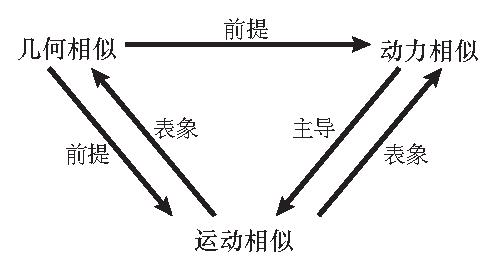
\includegraphics[scale=0.65]{figures/三种相似.eps}
	\caption{三种相似之间的关系}
\end{figure}

\LevelTwoTitle{准则数(2021·简答)}

\begin{enumerate}
	\item 雷诺数,惯性力与粘性力之比,适用于粘性流动,例如完全充满的管道内流动,数学表达为
	\begin{equation}
		Re = \dfrac{\rho V L}{\mu}
	\end{equation}
    \item 弗劳德数,惯性力和重力之比,适用于含有自由面的流动,例如明渠流、船舶形成的波运动,数学表达为
    \begin{equation}
    	Fr = \dfrac{V}{\sqrt{gL}}
    \end{equation}
    \item 欧拉数,压力与惯性力之比,适用于压力对流速分布影响较大的流动,例如空化效应,数学表达为
    \begin{equation}
    	Eu = \dfrac{\Delta p}{\rho V^2}
    \end{equation}
    \item 马赫数,惯性力和弹性力之比,适用于可压缩高速流动,例如加速喷管,数学表达为
    \begin{equation}
    	Ma = \dfrac{v}{a}
    \end{equation}
\end{enumerate}

需要掌握这四个准则数,韦伯数$We$和斯特劳哈尔数$Sr$了解即可。

\LevelTwoTitle{*近似模型法}

\LevelThreeTitle{什么是近似模型法}

\begin{definition}[近似模型法]
	保证模型流动和实物流动部分相似的方法,所谓“部分相似”,是指起主要作用的准则数相等。
\end{definition}

\LevelThreeTitle{雷诺相似}

适用于管道流动、物体绕流等,要求是:无自由面,重力对流态无影响,流速不高,可视作不可压缩流动,只考虑粘性力和压力,特征速度不能太大(太大将会影响压缩性)

\LevelThreeTitle{弗劳德相似}

适用于明渠流、船舶运动等,要求是:尺度不能太小,忽略表面张力,可视作不可压缩流动,粘性影响可以忽略或处于自模化状态,特征长度不能太小(太小将会影响粘性)

\LevelThreeTitle{什么是自模化}

\begin{definition}[自模化]
	流动相似本来取决于某准则数相等,但当其大到或小到一定程度时,即使准则数不等,流动也是相似的,这种状态就叫自模化。
\end{definition}

\LevelOneTitle{势流}

\LevelTwoTitle{涡量和旋转角速度}

\begin{enumerate}
	\item 涡量
	\begin{equation}
		\vec{\Omega} = \nabla \times \vec{V}
	\end{equation}
    \item 旋转角速度
    \begin{equation}
    	\vec{\omega} = \dfrac{1}{2} \vec{\Omega} = \dfrac{1}{2} \nabla \times \vec{V}
    \end{equation}
\end{enumerate}

\begin{definition}[势流]
	涡量为零或旋转角速度为零的流动称为势流,简单地讲,无旋必有势,即
	\begin{equation}
		\vec{\Omega} = 0 \text{~或~} \vec{\omega} = 0
	\end{equation}
\end{definition}

对于理想不可压缩流动,初始无旋,始终无旋;来流无旋,全场无旋。

\LevelTwoTitle{速度势函数}

速度势函数用$\phi$表示,存在条件是无旋,它满足

\begin{equation}
	\dd{\phi} = u\dd{x} + v\dd{y} + w\dd{z} = \pdv{\phi}{x} \dd{x} + \pdv{\phi}{y} \dd{y} + \pdv{\phi}{z} \dd{z}
\end{equation}

即

\begin{equation}
	\nabla \phi = \vec{V}
\end{equation}

速度势函数有无数个表达式(任意加上常数不影响速度分布),速度沿曲线的线积分与路径无关,任意封闭曲线的速度环量为零。

不可压流动势函数满足拉普拉斯方程

\begin{equation}
	\nabla^2 \phi = \pdv[2]{\phi}{x} + \pdv[2]{\phi}{y} + \pdv[2]{\phi}{z}= 0
\end{equation}

注意柱坐标系下的表达式
\begin{align*}
	&\dd{\phi} = V_r \dd{r} + rV_{\theta} \dd{\theta} + V_z \dd{z}\\
	&\nabla\phi = \pdv{\phi}{r}e_r + \dfrac{\partial \phi}{r \theta} e_{\theta} + \pdv{\phi}{z} e_z\\
	&\nabla^2 \phi = \dfrac{1}{r} \pdv{r}\qty(r\pdv{\phi}{r}) + \dfrac{\partial^2 \phi}{r^2 \partial \theta^2} + \pdv[2]{\phi}{z} = 0
\end{align*}

\LevelTwoTitle{势流伯努利方程}

\begin{equation}
	\dfrac{p}{\rho} + \dfrac{V^2}{2} + gz = \text{const}
\end{equation}

各项物理意义可以参考流线伯努利方程,总体物理意义是流体机械能在全流场守恒,且为同一常数。

适用条件

\begin{enumerate}
	\item 理想不可压流体;
	\item 定常;
	\item 质量力仅有重力或可以忽略;
	\item 无旋流动;
	\item 适用于整个流场
	\item 无其他能量输入输出。
\end{enumerate}

\begin{tip}
	势流伯努利方程与流线伯努利方程在形式上相同,但应注意,流线伯努利方程中的const对于不同流线是不同的,而势流伯努利方程中的const对全流场都相同。
\end{tip}

\LevelTwoTitle{平面势流}

\LevelThreeTitle{平面流动}

\begin{definition}[平面流动]
	任意时刻流场中各流体质点速度平行于某固定平面,各物理量在此平面上的垂直方向上不变化,数学表达为
	\begin{equation}
		\begin{split}
			&u_z = w = 0\\
			&\pdv{z} = 0
		\end{split}
	\end{equation}
\end{definition}

\LevelThreeTitle{平面势流}

\begin{equation}
	\omega_z \equiv 0 \text{~或~} \pdv{v}{x} - \pdv{u}{y} \equiv 0
\end{equation}

平面势流控制方程

\begin{enumerate}
	\item 连续方程(不可压)
	\begin{equation}
		\nabla \cdot \vec{V} = \pdv{u}{x} + \pdv{v}{y} = 0
	\end{equation}
    \item 运动方程(欧拉方程)
    \begin{equation}
    	\dfrac{\mathrm{D} \vec{V}}{\mathrm{D} t} = \vec{g} - \dfrac{1}{\rho} \nabla p
    \end{equation}
    \item 势流伯努利方程
\end{enumerate}

\LevelTwoTitle{流函数}

流函数用$\varPsi$表示,存在条件是二元不可压缩,它满足

\begin{equation}
	\dd{\psi} = -v\dd{x} + u\dd{y} = \pdv{\psi}{x} \dd{x} + \pdv{\psi}{y} \dd{y}
\end{equation}

流函数有无数个表达式(任意加上常数不影响速度分布),等流函数线就是二元流动的流线,流经任意曲线的流量等于曲线端点流函数之差,即$Q_{AB} = \psi_{B} - \psi_{A}$,若该曲线本身是流线,则$Q_{AB} = 0$。

势流条件下,流函数满足拉普拉斯方程

\begin{equation}
	\nabla^2 \psi = \pdv[2]{\psi}{x} + \pdv[2]{\psi}{y} = 0
\end{equation}

\begin{table}[H]
	\centering
	\begin{tabular}{ccc}
		\toprule[1pt]
		 & 速度势函数 & 流函数 \\
		 \hline
		存在条件 & 无旋(有势) & 不可压 \\
		\hline
		满足拉普拉斯方程条件 & 不可压 & 无旋(有势)\\
		\bottomrule[1pt]
	\end{tabular}
    \caption{存在和满足拉普拉斯方程条件总结}
\end{table}

\LevelTwoTitle{*流网}

令$\phi = \text{const}$,$\psi = \text{const}$,则得到等势线,满足

\begin{equation}
	\begin{split}
		&\dd{\phi} = u\dd{x} + v\dd{y} = 0\\
		&\dd{\psi} = -v\dd{x} + u\dd{y} = 0
	\end{split}
\end{equation}

等势线和流线斜率之积

\begin{equation*}
	\qty(\dv{y}{x})_{\phi} \cdot \qty(\dv{y}{x})_{\psi} = -\dfrac{u}{v} \cdot \dfrac{v}{u} = -1
\end{equation*}

这表明等势线和流线处处相互垂直,它们合起来组成流网。

\LevelTwoTitle{基本平面势流}

\begin{tip}
	可能会出叠加的计算题,但应该会给公式,下面仅列出速度势函数和流函数公式,由此可自行推出速度分布,再由平面势流伯努利方程可以得到压强分布。
\end{tip}

\begin{enumerate}
	\item 均直直线流动
	\begin{align*}
		&\phi = ax + by\\
		&\psi = -bx + ay
	\end{align*}
    \item 点源点汇
    \begin{align*}
    	&\phi = \pm \dfrac{m}{2\pi} \ln r\\
    	&\psi = \pm \dfrac{m}{2\pi} \theta
    \end{align*}
    其中,$m = \pm Q$为体积流量,外流为正(点源),内流为负(点汇)
    \item 点涡
    \begin{align*}
    	&\phi = \pm \dfrac{\varGamma}{2\pi} \theta\\
    	&\psi = \mp \dfrac{\varGamma}{2\pi} \ln r
    \end{align*}
    其中,$\varGamma = 2\pi K$为点涡强度,逆时针为正,顺时针为负。
    \item 偶极流,点源与点汇合成,由点汇指向点源为正。
\end{enumerate}

\begin{figure}[H]
	\centering
	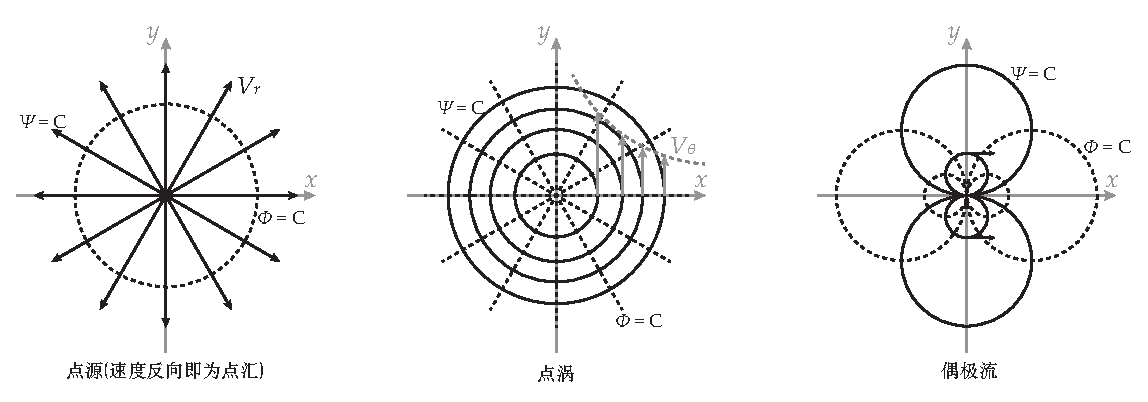
\includegraphics[scale=0.6]{figures/点源点涡偶极流.eps}
	\caption{点源、点涡和偶极流的流线和等势线}
\end{figure}

\LevelTwoTitle{*圆柱绕流}

\LevelThreeTitle{无环量圆柱绕流}

由$\vec{x}$方向均匀来流和$-\vec{x}$方向偶极流叠加而成,圆柱表面速度分布

\begin{align*}
	&V_r = 0\\
	&V_{\theta} = -2U \sin \theta 
\end{align*}

\begin{enumerate}
	\item $\theta = 0, \pi$,驻点;
	\item $\theta = \pm \dfrac{\pi}{2}$,舷点。
\end{enumerate}

\begin{figure}[H]
	\centering
	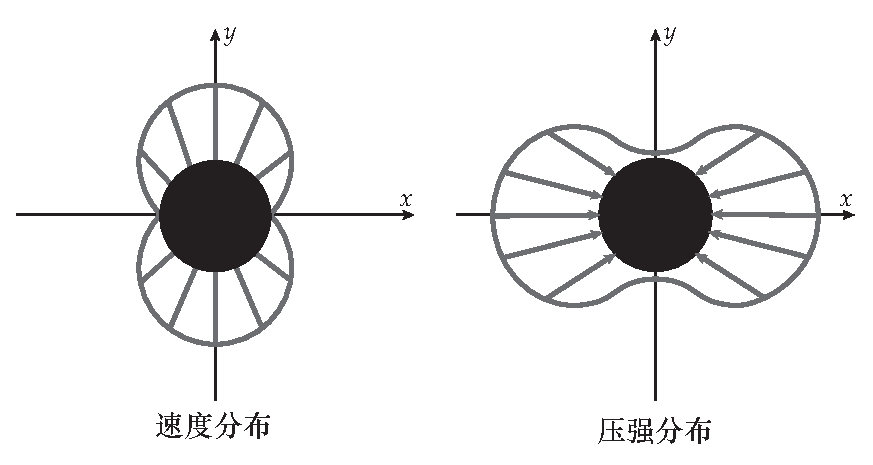
\includegraphics[scale=0.7]{figures/无环量.eps}
	\caption{无环量圆柱绕流的速度分布和压强分布}
\end{figure}

\LevelThreeTitle{有环量圆柱绕流}

由无环量圆柱绕流和点涡叠加而成,圆柱表面速度分布

\begin{align*}
	&V_r = 0\\
	&V_{\theta} = -2U \sin \theta \pm \dfrac{\varGamma}{2\pi R}
\end{align*}

$V_{\theta}$第二项,顺时针取负,逆时针取正。令其等于零,得驻点表达式$\sin \theta_s = \pm \dfrac{\varGamma}{4\pi R U}$,关于驻点个数讨论如下

\begin{enumerate}
	\item $\varGamma < 4\pi R U$,2个;
	\item $\varGamma = 4\pi R U$,1个;
	\item $\varGamma > 4\pi R U$,0个。
\end{enumerate}

\begin{figure}[H]
	\centering
	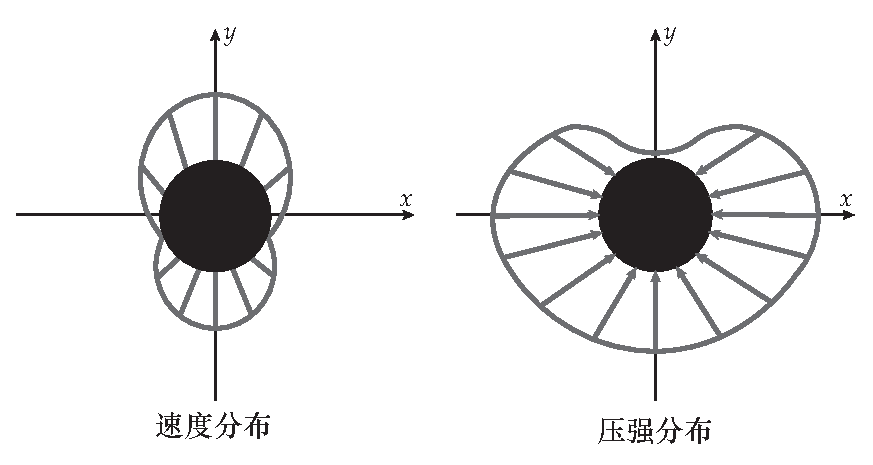
\includegraphics[scale=0.7]{figures/有环量.eps}
	\caption{有环量圆柱绕流的速度分布和压强分布}
\end{figure}

\LevelThreeTitle{达朗贝尔悖论}

理想不可压缩流动中任一封闭物体绕流阻力为零,产生此悖论的原因是没有考虑粘性。

\LevelTwoTitle{例题练习}

\begin{example}
	试证明$\psi = x + 2x^2 - 2y^2$所表示的流动是势流,并求出该流动的速度势函数。若流体的密度是1.21 kg/m$^3$,在点$(1, -2)$处压强$p = 4.8$ kPa,试求点$(9, 6)$处的压强。
	
	\begin{equation*}
		\nabla^2 \psi = \pdv[2]{\psi}{x} + \pdv[2]{\psi}{y} = 4 - 4 = 0
	\end{equation*}
    故该流动是势流。
    \begin{equation*}
    	u = \pdv{\psi}{y} = \pdv{\phi}{x} = -4y, ~v = -\pdv{\psi}{x} = \pdv{\phi}{y} = -1 - 4x
    \end{equation*}
    于是
    \begin{equation*}
    	\phi = \int -4y \dd{x} + f(y) = -4xy + f(y)
    \end{equation*}
    求导
    \begin{equation*}
    	\pdv{\phi}{y} = -4x + f'(y) = v
    \end{equation*}
    对比,得
    \begin{equation*}
    	f'(y) = -1 \Rightarrow f(y) = -y + C
    \end{equation*}
    故$\phi = -4xy - y + C$。
    速度分布
    \begin{equation*}
    	\vec{V} = u \vec{i} + v \vec{j}
    \end{equation*}
    则$(1, -2)$点处$V_1^2 = 89 \mathrm{~m}^2 / \mathrm{s}^2$,$(9, 6)$点处$V_2^2 = 1945 \mathrm{~m}^2 / \mathrm{s}^2$。
    
    列伯努利方程
    \begin{equation*}
    	\dfrac{p_1}{\rho} + \dfrac{V_1^2}{2} = \dfrac{p_2}{\rho} + \dfrac{V_2^2}{2}
    \end{equation*}
    解得
    \begin{equation*}
    	p_2 = 3.76 \mathrm{~kPa}
    \end{equation*}
\end{example}

\begin{tip}
	2021年计算题第一道跟本题类似,需要对速度、速度势函数和流函数之间的关系很清楚。叠加类题目考的概率比较小,若要练习可以参考课后题8.13 ~ 8.21。
\end{tip}


\LevelOneTitle{管道内流动}

\LevelTwoTitle{圆管湍流特性}

\begin{figure}[H]
	\centering
	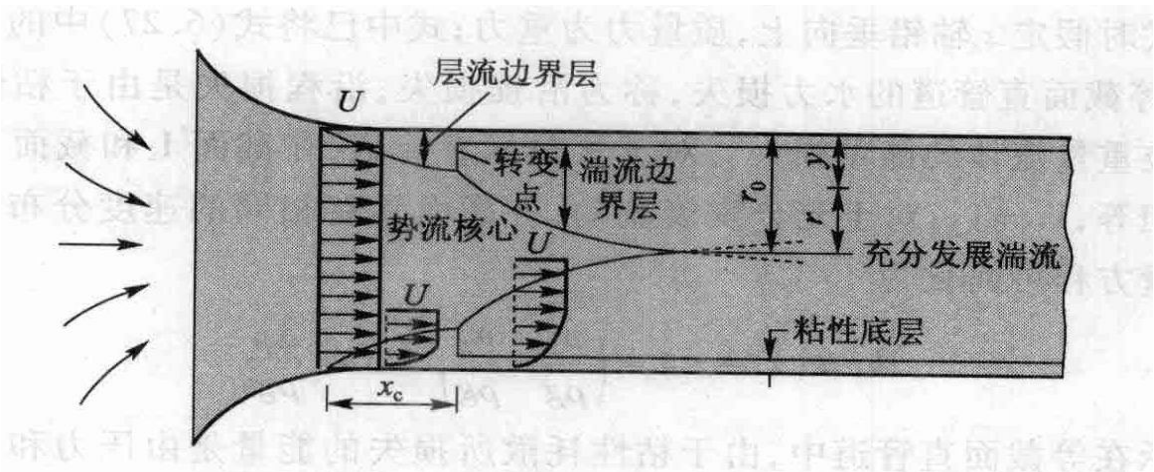
\includegraphics[scale=0.3]{figures/圆管湍流.png}
	\caption{圆管湍流示意}
\end{figure}

势流核心区短,粘性区域厚度增加快,达到充分发展需要的长度长,充分发展段:速度分布更均匀,沿流动方向速度分布不变,过流断面上切应力分布相同,速度分布相同,压降与$x$成线性关系(单位压降相同),压力(有时也有重力)和粘性力平衡。

$Re$增大,起始段长度增加,充分发展段速度分布更均匀。

\LevelTwoTitle{实际总流伯努利方程}

\begin{equation}
	\dfrac{\alpha_1 \overline{V}_1^2}{2g} + z_1 + \dfrac{p_1}{\rho g} = \dfrac{\alpha_2 \overline{V}_2^2}{2g} + z_2 + \dfrac{p_2}{\rho g} + h_f + h_{\text{轴}}
\end{equation}

式中$\alpha$的取值需要根据流态确定,$Re > Re_{cr} = 2300$,湍流,$\alpha = 1$;$Re < Re_{cr} = 2300$,层流,$\alpha = 2$(考试一般都是湍流,但仍需要先判断再取值)。

物理意义可以参照总流伯努利方程来写,注意加上水里损失和轴功影响。

适用条件:

\begin{enumerate}
	\item 不可压缩流动;
	\item 定常;
	\item 质量力有势且只有重力;
\end{enumerate}

\LevelTwoTitle{水力损失和轴功}

\begin{definition}[水力损失$h_f$]
	单位重量流体由1点流到2点克服粘性力损失的能量(机械能),分为沿程阻力损失$h_l$和局部阻力损失$h_m$,即$h_f = \sum h_l + \sum h_m$。
\end{definition}

\LevelThreeTitle{圆管沿程阻力损失}

沿程阻力损失是流体在均直管道内克服摩擦阻力做功,损失的能量可能来自压力能(水平管道)和重力势能(非水平管道),数学表达为

\begin{equation}
	h_l = f \dfrac{l}{D} \dfrac{\overline{V}^2}{2g} \label{eq9.2}
\end{equation}

其中,

\begin{enumerate}
	\item 圆管层流,$f = \dfrac{64}{Re}$;
	\item 圆管湍流,$f = 0.11\qty(\dfrac{68}{Re} + \dfrac{\Delta}{D})^{0.25}$(水力粗糙);$f = \dfrac{0.3164}{Re^{0.25}}$(*水力光滑)。
\end{enumerate}

\LevelThreeTitle{非圆管沿程阻力损失}

只需令式\ref{eq9.2}中$f = \dfrac{C}{Re_h}$和$D \to D_h = \dfrac{4A}{P}$即可。

其中,$C$与截面形状尺寸有关,$D_h$称为当量直径(水力直径),$A$为过流断面面积,$P$为湿周,是粘性应力作用的所有周长。

\begin{tip}
	此处可能考选择题,考查水力直径、湿周的定义等,计算大题应该还是圆管。
\end{tip}

\LevelThreeTitle{局部阻力损失(2021·简答)}

局部阻力损失是经过各种管道构件和管道连接件产生的损失,具体原因是发生了速度场突变、流体元碰撞,甚至是流体分离形成旋涡,数学表达为

\begin{equation}
	h_m = K\dfrac{\overline{V}^2}{2g}
\end{equation}

其中,$K$取决于管件几何形状、尺寸和流动的$Re$,当$Re$很大时,$K$与$Re$无关。题目中一般会给$K$的值,但仍建议记忆出入口处的$K$值。

\begin{enumerate}
	\item $A_2 \gg A_1$,$K = 1$;
	\item $A_1 \gg A_2$,$K = 0.5$。
\end{enumerate}

大口变小口损失小,小口变大口损失大。

\LevelThreeTitle{轴功}

\begin{enumerate}
	\item $h_{\text{轴}} < 0$,表明机械向流体作功,例如水泵;
	\item $h_{\text{轴}} > 0$,表明流体向机械作功,例如水轮机;
	\item 功率$\dot{W} = \rho g Q \abs{h_{\text{轴}}}$。
\end{enumerate}

\LevelTwoTitle{*穆迪图的四个区域}

\begin{enumerate}
	\item 层流区,$f = \dfrac{64}{Re}$;
	\item 水力光滑区,$f = f(Re)$;
	\item 过渡粗糙区,$f = f(Re, \dfrac{\Delta}{D})$;
	\item 完全粗糙区,$f = f(\dfrac{\Delta}{D})$。
\end{enumerate}

\LevelTwoTitle{串、并联管道}

\begin{enumerate}
	\item 串联
	\begin{align*}
		&Q_1 = Q_2 = Q_3 = \cdots\\
		&h_f = \sum h_{f_i}
	\end{align*}
    \item 并联
    \begin{align*}
    	&Q = \sum Q_i\\
    	&h_{f_1} = h_{f_2} = h_{f_3} = \cdots
    \end{align*}
\end{enumerate}

\LevelTwoTitle{例题练习}

\begin{example}
	如图,运动粘度$\nu = 5.16 \times 10^{-6}$ m$^2$/s,密度$\rho = 861$ kg/m$^3$的燃油通过长1830 m,内径为$d = 400$ mm的铆接钢管($\varepsilon = 2$ mm)输送到油池C。流量为0.2 m$^3$/s时,A点表压为13.8 kPa。试求泵AB的输出功率和B点的压强,忽略局部阻力损失。
	
	\begin{figure}[H]
		\centering
		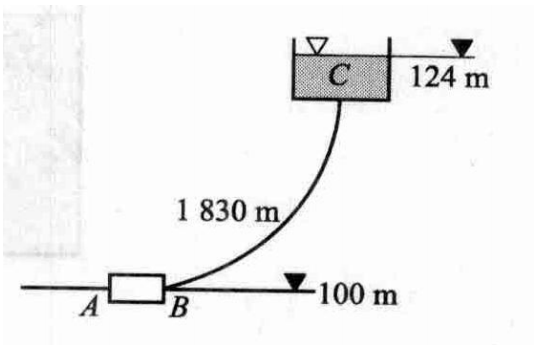
\includegraphics[scale=0.4]{figures/C9-fig1.png}
		\caption{例图}
	\end{figure}

    \begin{enumerate}
    	\item 雷诺数
    	\begin{equation*}
    		Re = \dfrac{Vd}{\nu} = \dfrac{4Q}{\pi \nu d} = \dfrac{4 \times 0.2}{\pi \times 5.16 \times 10^{-6} \times 0.4} = 123376 \gg 2300
    	\end{equation*}
        故该流动为湍流,动能修正系数$\alpha = 1$。
        \item 沿程阻力损失
        \begin{align*}
        	&f = 0.11 \qty(\dfrac{68}{Re} + \dfrac{\varepsilon}{d})^{0.25} = 0.11 \times \qty(\dfrac{68}{123376} + \dfrac{2}{400})^{0.25} = 0.03\\
        	&h_l = f \dfrac{l}{d} \dfrac{V^2}{2g} = f \dfrac{l}{d} \dfrac{8Q^2}{\pi^2 d^4 g} = 0.03 \times \dfrac{1830}{0.4} \times \dfrac{8 \times 0.2^2}{\pi^2 \times 0.4^4 \times 9.8} \mathrm{~m} = 17.74 \mathrm{~m}
        \end{align*}
        \item 取A,C两处列伯努利方程
        \begin{equation*}
        	\dfrac{V^2}{2g} + z_A + \dfrac{p_A}{\rho g} = \dfrac{V^2}{2g} + z_C + 0 + h_l + h_{\text{轴}}
        \end{equation*}
        解得
        \begin{equation*}
        	h_{\text{轴}} = -40.10 \mathrm{~m} < 0
        \end{equation*}
        表明流体机械向流体输出功。
        \item 泵AB输出功率
        \begin{equation*}
        	\dot{W} = \rho g Q \abs{h_{\text{轴}}} = 861 \times 9.8 \times 0.2 \times 40.10 \times 10^{-3} \mathrm{~kW} = 67.67 \mathrm{~kW}
        \end{equation*}
        \item 对A,B处,由伯努利方程
        \begin{equation*}
        	\dfrac{p_A}{\rho g} = \dfrac{p_B}{\rho g} + h_{\text{轴}}
        \end{equation*}
        解得
        \begin{equation*}
        	p_B = 352.2 \mathrm{~kPa}
        \end{equation*}
    \end{enumerate}
\end{example}

\begin{tip}
	考试中本章必涉及一道计算,并且会考虑局部阻力损失(本题没有考虑),可以参考课后习题9.25掌握局部阻力损失的计算。
\end{tip}


\LevelOneTitle{绕物体的粘性不可压流动}

\begin{tip}
	2021年春的期末考试题中没有任何一道题涉及本章知识。
\end{tip}

\LevelTwoTitle{边界层}

\begin{definition}[边界层]
	高$Re$流动时,贴近固体壁面附近的速度梯度很大,粘性影响不能忽略且流动有旋的薄层。
\end{definition}

\LevelTwoTitle{三种厚度}

\begin{enumerate}
	\item 边界层厚度\\
	由壁面沿外法线到速度达到99\%的距离,随流动方向增大,反映了粘性影响和旋涡扩散范围,数学表达为
	\begin{equation}
		\dfrac{u}{U} = 0.99 \Rightarrow y = \delta
	\end{equation}
    \item *位移(排挤)厚度\\
    实际断面流量较理想流动的减少量可以看作壁面向流体方向移动的距离,反映了边界层对主流区的影响程度,数学表达为
    \begin{equation}
    	\delta^{*} = \int_{0}^{\delta} \qty(1 - \dfrac{u}{U}) \dd{y}
    \end{equation}
    \item *动量损失厚度\\
    实际断面流体动量较理想流动的减少量可以看作壁面向流体方向移动的距离,动量损失厚度越大,流体的动量损失就越大,数学表达为
    \begin{equation}
    	\theta = \int_{0}^{\delta} \dfrac{u}{U}\qty(1 - \dfrac{u}{U}) \dd{y}
    \end{equation}
\end{enumerate}

通常情况下,有$\delta > \delta^{*} > \theta$。

\LevelTwoTitle{边界层内的流动}

\LevelThreeTitle{流态判断}

有两个雷诺数用于判断流态,$x$是距前缘的距离,$\delta$是边界层厚度。

\begin{equation*}
	Re_{x} = \dfrac{Ux}{\nu}, Re_{\delta} = \dfrac{U\delta}{\nu}
\end{equation*}

\LevelThreeTitle{*流动特征}

边界层流动主要有以下特征:

\begin{enumerate}
	\item 与流动问题特征长度相比,厚度很小;
	\item 沿流动方向厚度增加,边界层边缘不与流线重合;
	\item 沿壁面法线方向速度梯度很大;
	\item 粘性力和惯性力是同一数量级的;
	\item 有旋,沿壁面法向各点压强相等;
	\item 存在层流、湍流两种流态。
\end{enumerate}

\LevelTwoTitle{顺流平板的绕流}

\begin{enumerate}
	\item 边界层方程
	\begin{equation}
		\dv{\theta}{x} = \dfrac{\tau_{w}}{\rho U^2}
	\end{equation}
    \item 阻力公式
    \begin{equation}
    	F_D = C_D \dfrac{1}{2} \rho U^2 A
    \end{equation}
\end{enumerate}

\LevelThreeTitle{层流边界层}

\begin{enumerate}
    \item 边界层厚度
    \begin{equation}
    	\delta = 5.0 \sqrt{\dfrac{\mu x}{\rho U}}
    \end{equation}
    \item 阻力系数
    \begin{equation}
    	C_D = \dfrac{1.328}{\sqrt{Re_L}}
    \end{equation}
\end{enumerate}

\LevelThreeTitle{湍流边界层}

\begin{enumerate}
	\item 边界层厚度
	\begin{equation}
		\delta = 0.37 \dfrac{x}{Re_x^{0.2}}
	\end{equation}
	\item 阻力系数
	\begin{enumerate}
		\item $5 \times 10^5 \leq Re_L \leq 10^7$时,
		\begin{equation}
			C_D = \dfrac{0.074}{Re_L^{0.2}}
		\end{equation}
	    \item $10^7 \leq Re_L \leq 10^9$时,
	    \begin{equation}
	    	C_D = \dfrac{0.455}{\qty(\lg Re_L)^{2.58}}
	    \end{equation}
	\end{enumerate}
\end{enumerate}

\LevelThreeTitle{*混合边界层}

\begin{enumerate}
	\item 转捩临界长度
	\begin{equation}
		x_{cr} = \dfrac{Re_{cr} \nu}{U}
	\end{equation}
    $L < x_{cr}$($Re_L < Re_{cr}$),平板边界层为层流边界层,$L > x_{cr}$($Re_L > Re_{cr}$)为混合边界层。
    \item 阻力简单模型:全部湍流-$x_{cr}$之前湍流+$x_{cr}$之前层流
    \begin{enumerate}
    	\item $Re_L \leq 10^7$时,
    	\begin{equation}
    		F_D = \dfrac{1}{2} \rho U^2 b \qty[\dfrac{0.074}{Re_L^{0.2}} L - \dfrac{0.074}{Re_L^{0.2}} x_{cr} + \dfrac{1.328}{\sqrt{Re_L}} x_{cr}]
    	\end{equation}
    	\item $10^7 < Re_L < 10^9$时,
    	\begin{equation}
    		F_D = \dfrac{1}{2} \rho U^2 b \qty[\dfrac{0.455}{\qty(\lg Re_L)^{2.58}} L - \dfrac{0.074}{Re_L^{0.2}} x_{cr} + \dfrac{1.328}{\sqrt{Re_L}} x_{cr}]
    	\end{equation}
    \end{enumerate}
\end{enumerate}

\LevelTwoTitle{曲壁边界层分离}

曲壁边界层分离必要条件是

\begin{enumerate}
	\item 固体壁面;
	\item 逆压梯度$\displaystyle \pdv{p}{x} > 0$(压力合力与流速方向相反,与粘性力合力方向相同,发生回流);
	\item 粘性流体。
\end{enumerate}

分离点满足

\begin{equation}
	\eval{\pdv{u}{y}}_{y = 0} = 0
\end{equation}

\LevelTwoTitle{例题练习}

\begin{example}
	一长为2.4 m,宽为0.9 m的光滑矩形平板沿长边方向以6 m/s的速度在静止空气中运动,已知空气密度为1.21 kg/m$^3$,运动粘度$\nu = 14.9$ mm$^2$/s。假定平板边界层全为层流,试计算平板后缘边界层的厚度以及使平板运动所需要的功率。若平板边界层全为湍流,功率为多大?
	
	\begin{enumerate}
		\item 若为层流边界层,则
		\begin{equation*}
			\delta = 5\sqrt{\dfrac{\nu L}{U}} = 5\sqrt{\dfrac{14.9 \times 10^{-6} \times 2.4}{6}} \mathrm{~m} = 0.01221 \mathrm{~m}
		\end{equation*}
	    又
	    \begin{equation*}
	    	Re_L = \dfrac{UL}{\nu}, ~C_D = \dfrac{1.328}{Re_L}
	    \end{equation*}
        则两侧摩擦阻力
        \begin{align*}
        	F_D &= 2C_D \cdot \dfrac{1}{2} \rho U^2 \cdot bL\\
        	&= 2\times \dfrac{1.328}{\sqrt{\dfrac{6 \times 2.4}{14.9 \times 10^{-6}}}} \times \dfrac{1}{2} \times 1.21 \times 6^2 \times 0.9 \times 2.4 \mathrm{~N}\\
        	&= 0.1271 \mathrm{~N}
        \end{align*}
        所需功率
        \begin{equation*}
        	\dot{W} = F_D \cdot U = 0.1271 \times 6 \mathrm{~W} = 0.7626 \mathrm{~W}
        \end{equation*}
        \item 若为湍流边界层,则$C_D = \dfrac{0.0742}{(Re_L)^{0.2}}$,同样的计算方法解得$\dot{W} = 2.661 \mathrm{~W}$。
	\end{enumerate}
\end{example}


\LevelOneTitle{可压缩流动基础}

\LevelTwoTitle{微弱扰动波}

\LevelThreeTitle{*什么是微弱扰动波}

\begin{definition}[微弱扰动波]\label{def11.1}
	由扰动源发出的,通过介质后状态发生微弱变化的波,其传播过程可视作一等熵过程。
\end{definition}

\LevelThreeTitle{什么是音速}

\begin{definition}[音速]
	微弱扰动波在可压缩介质中传播的速度(相对于流体介质),用$a$表示。
\end{definition}

\begin{equation}
	a = \sqrt{\dv{p}{\rho}} = \sqrt{\dfrac{E_v}{\rho}} = \sqrt{\gamma R_g T}
\end{equation}

\LevelThreeTitle{什么是马赫数}

\begin{definition}
	流速与当地音速之比,物理意义是惯性力和弹性力之比,即
	\begin{equation}
		Ma = \dfrac{V}{a}
	\end{equation}
\end{definition}

\LevelThreeTitle{微弱扰动波的传播区域}

\begin{figure}[H]
	\centering
	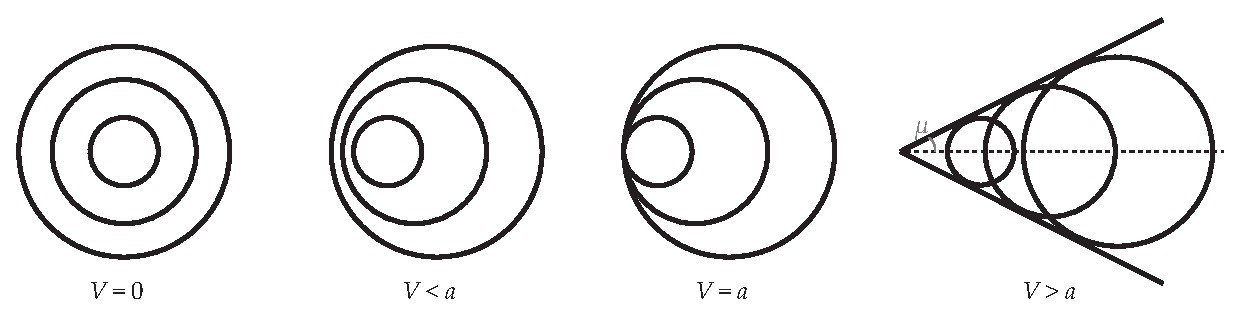
\includegraphics[scale=0.7]{figures/微弱扰动波.eps}
	\caption{微弱扰动波传播的区域}
\end{figure}

当$V > a$时,流体超音速,形成马赫角$\mu$,数学表达为

\begin{equation*}
	\mu = \arcsin(\dfrac{a}{V}) = \arcsin(\dfrac{1}{Ma})
\end{equation*}

\LevelTwoTitle{定常一元等熵流动控制方程组}

\begin{align*}
	&\rho V A = \text{const}\\
	&h + \dfrac{V^2}{2} = \text{const}\\
	&p = \rho R_g T\\
	&\dfrac{p}{\rho^{\gamma}} = \text{const}
\end{align*}

\LevelTwoTitle{三种参考状态}

\begin{enumerate}
	\item 等熵滞止状态\\
	速度滞止为零时的状态,$h_0 = h + \dfrac{V^2}{2} \Rightarrow T_0 = T + \dfrac{V^2}{2 c_p}$。
	\item 临界状态\\
	流速达到音速的状态($Ma = 1$),$T^{*} = 0.833 T_0, p^{*} = 0.528 p_0$。
	\item 极限状态\\
	温度为0 K,流速达到最大,$V_{\text{max}} = \sqrt{2h_0}$
\end{enumerate}

\LevelTwoTitle{速度系数和喷管}

\LevelThreeTitle{速度系数}

速度系数$\lambda = \dfrac{V}{a^{*}}$,物理意义是直接反映当地速度大小。

\LevelThreeTitle{喷管}

喷管的流动工况和截面变化之间的关系

\begin{equation}
	(Ma^2 - 1) \dfrac{\dd{V}}{V} = \dfrac{\dd{A}}{A}
\end{equation}

例如,当流动超音速($Ma^2 - 1 > 0$),想要让出口流速减小($\dfrac{\dd{V}}{V} < 0$),则应选择渐缩喷管($\dfrac{\dd{A}}{A} < 0$)。

喷管内流动参数变化,若$V\uparrow$,则$T, \rho, p\downarrow$;流速增大则相反,其中$p$的变化最剧烈。

\begin{enumerate}
	\item 渐缩喷管
	\begin{enumerate}
		\item $p_b \geq p^{*} \Rightarrow p_e = p_b$;
		\item $p_b < p^{*} \Rightarrow p_e = p^{*}$。
	\end{enumerate}
    \item 缩放喷管,$p_b < p^{*} \Rightarrow p_e = p_b$
\end{enumerate}

\LevelThreeTitle{个人比较喜欢的一个公式}

\begin{equation}
	\dfrac{p_e}{p_0} = \qty(1 + \dfrac{\gamma - 1}{2} Ma_e^2)^{-\frac{\gamma}{\gamma - 1}}
\end{equation}

\LevelTwoTitle{激波}

\LevelTwoTitle{*什么是激波}

\begin{definition}[激波]
	集中的有一定强度的压缩波称为激波,是由于传播速度超音速发生突跃压缩现象产生的,强间断且具有一定厚度,激波内速度梯度和温度梯度很大。
\end{definition}

\LevelThreeTitle{激波的分类}

\begin{enumerate}
	\item 正激波,波面与气流方向垂直;
	\item 斜激波,波面与气流方向不垂直;
	\item 曲面激波,波形弯曲,由正激波和斜激波构成。
\end{enumerate}

\LevelTwoTitle{正激波前后参数变化}

\begin{equation*}
	V_1 V_2 = {a^{*}}^2 \Rightarrow \lambda_1 \lambda_2 = 1
\end{equation*}

\begin{enumerate}
	\item 静参数变化\\
	$V, Ma \downarrow, T, p, \rho, a \uparrow$;
	\item 滞止参数变化\\
	$T_0$不变,$p, \rho \downarrow$;
	\item 临界参数变化\\
	$T^{*}$不变,$p, \rho \downarrow$。
\end{enumerate}

\LevelTwoTitle{例题练习}

\begin{example}
	一真空箱通过收缩形喷管从大气吸气,喷管最小截面直径为38 mm,若大气压强为101.3 kPa,温度为15 $^{\circ}$C,要使喷管出口为音速流动,真空箱压强应保持为多少?此时质量流量多少?若真空箱内压强为$0.34 \times 10^5$ Pa,质量流量为多少?
	\vskip 0.3cm
	由于是从大气吸气,因此入口参数为滞止参数,则
	\begin{equation*}
		p^{*} = 0.528 p_0 = 0.528 \times 101.3 \mathrm{~kPa} = 53.486 \mathrm{~kPa}
	\end{equation*}

	由题意,$V_e = a^{*}$,则$p_e = p^{*} = p_b$。	
	\vskip -0.3cm
    \begin{align*}
    	&T^{*} = 0.833 T_0 = 0.833 \times (15 + 273.15) \mathrm{~K} = 240 \mathrm{~K}\\
    	&\rho^{*} = \dfrac{p^{*}}{R_g T^{*}} = \dfrac{53.486 \times 10^3}{287 \times 240} \mathrm{~kg/m}^3 = 0.7765 \mathrm{~kg/m}^3\\
		&a^{*} = \sqrt{\gamma R_g T} = \sqrt{1.4 \times 287 \times 240} \mathrm{~m/s} = 310.5 \mathrm{~m/s}\\
		&\dot{m} = \rho^{*} A_e a^{*} = \dfrac{\pi \rho^{*} d_e^2 a^{*}}{4} = \dfrac{\pi \times 0.7765 \times 0.038^2 \times 310.5}{4} \mathrm{~kg/s} = 0.2734 \mathrm{~kg/s}
	\end{align*}

	若$p_b = 34$ kPa $< p^{*}$,则$p_e = p^{*}$,于是$\dot{m} = 0.2734 \mathrm{~kg/s}$不变。
\end{example}

\begin{example}
	大容器内温度为20 $^{\circ}$C的空气以1.2 kg/s的流量通过缩放喷管,喷管出口截面压强和马赫数分别是14 kPa和2.8,试确定喷管喉部和出口面积、喉部压强、出口气流速度。
	\vskip 0.3cm
	
	\begin{equation*}
		\dfrac{p_e}{p_0} = \qty(1 + \dfrac{\gamma - 1}{2} Ma_e^2)^{-\frac{\gamma}{\gamma - 1}} \Rightarrow p_0 = 379.94 \mathrm{~kPa}\\
	\end{equation*}
	
	由于$Ma_e > 1$,则喉部必达临界状态,喉部压强$p^{*} = 0.528 p_0 = 0.528 \times 379.94 \mathrm{~kPa}$。
	
	\begin{align*}
		&T_e = T_0\qty(\dfrac{p_e}{p_0})^{\frac{\gamma - 1}{\gamma}} = 290.15 \times \qty(\dfrac{14}{379.94})^{\frac{0.4}{1.4}} \mathrm{~K} = 112.99 \mathrm{~K}\\
		&a_e = \sqrt{\gamma R_g T_e} = \sqrt{1.4 \times 287 \times 112.99} \mathrm{~m/s} = 213.07 \mathrm{~m/s}\\
		&V_e = Ma_e \cdot a_e = 2.8 \times 213.07 \mathrm{~m/s} = 596.6 \mathrm{~m/s}\\
		&\rho_e = \dfrac{p_e}{R_g T} = \dfrac{14000}{287 \times 112.99} \mathrm{~kg/m}^3 = 0.4317 \mathrm{~kg/m}^3\\
		&A_e = \dfrac{\dot{m}}{\rho_e V_e} = \dfrac{1.2}{0.4317 \times 596.6} \mathrm{~m}^2 = 4.659 \times 10^{-3} \mathrm{~m}^2\\
		&T^{*} = T_0\qty(\dfrac{p^{*}}{p_0})^{\frac{\gamma - 1}{\gamma}} = 290.15 \times \qty(\dfrac{200.61}{379.94})^{\frac{0.4}{1.4}} \mathrm{~K} = 241.76 \mathrm{~K}\\
    	&\rho^{*} = \dfrac{p^{*}}{R_g T} = \dfrac{200610}{287 \times 241.76} \mathrm{~kg/m}^3 = 2.891 \mathrm{~kg/m}^3\\
    	&a^{*} = \sqrt{\gamma R_g T} = \sqrt{1.4 \times 287 \times 241.76} \mathrm{~m/s} = 311.67 \mathrm{~m/s}\\
    	&A_{\text{min}} = \dfrac{\dot{m}}{\rho^{*} a^{*}} = \dfrac{1.2}{2.891 \times 311.67} \mathrm{~m}^2 = 1.332 \times 10^{-3} \mathrm{~m}^2
    \end{align*}
\end{example}

\end{document}